\paragraph[QuizziPedia::Front-End::ModelViews\\::RegistrationManagementModelView]{QuizziPedia::Front-End::ModelViews::RegistrationManagementModelView}
	
	\label{QuizziPedia::Front-End::ModelViews::RegistrationManagementModelView}
	
	\begin{figure}[ht]
		\centering
		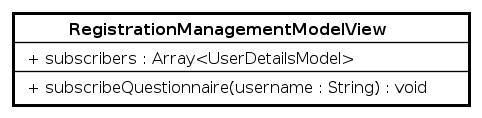
\includegraphics[scale=0.5,keepaspectratio]{UML/Classi/Front-End/QuizziPedia_Front-end_ModelView_RegistrationManagementModelView.png}
		\caption{QuizziPedia::Front-End::ModelViews::RegistrationManagementModelView}
	\end{figure} \FloatBarrier
	
	\begin{itemize}
		\item \textbf{Descrizione}: classe di tipo modelview la cui istanziazione è contenuta all'interno della variabile di ambiente \texttt{\$scope} di \textit{Angular\ped{G}}. All'interno di essa sono presenti le variabili e i metodi necessari per il \textit{Two-Way Data-Binding\ped{G}} tra la \textit{view\ped{G}} \texttt{RegistrationManagementView} e il \textit{controller\ped{G}} \texttt{RegistrationManagementController};
		\item \textbf{Utilizzo}: viene utilizzata per effettuare il \textit{Two-Way Data-Binding\ped{G}} tra la \textit{view\ped{G}}\\ \texttt{RegistrationManagementView} e il \textit{controller\ped{G}} \texttt{RegistrationManagementController} rendendo disponibili variabili e metodi;
		\item \textbf{Relazioni con altre classi}: 
		\begin{itemize}
			\item \textbf{IN \texttt{RegistrationManagementController}}: questa classe permette di gestire le iscrizione degli utenti ai questionari;
			\item \textbf{OUT \texttt{RegistrationManagementView}}: \textit{view\ped{G}} che permette di visualizzare gli utenti iscritti ad un questionario.
		\end{itemize}
		\item \textbf{Attributi}: 
		\begin{itemize}
			\item \texttt{+ subscribers: Array<UserDetailsModel>} \\ \texttt{array} contenente un oggetto per ogni utente iscritto al questionario. L'oggetto sarà composto dai campi \texttt{nome} e \texttt{cognome};
		\end{itemize}
		\item \textbf{Metodi}: 
		\begin{itemize}
			\item \texttt{+ subscribeQuestionnaire(username: String): void} \\ Metodo che permette l'iscrizione ad un questionario. Richiama la funzionalità del \texttt{QuizService}. \\
			\textbf{Parametri}:
			\begin{itemize}
				\item \texttt{username: String}\\
				Parametro che indica l'utente da iscrivere al questionario.
			\end{itemize}
		\end{itemize}
	\end{itemize}
	
	